%
% $RCSfile: portals_and_services.tex,v $
%
% Copyright (C) 2002-2008. Christian Heller.
%
% Permission is granted to copy, distribute and/or modify this document
% under the terms of the GNU Free Documentation License, Version 1.1 or
% any later version published by the Free Software Foundation; with no
% Invariant Sections, with no Front-Cover Texts and with no Back-Cover
% Texts. A copy of the license is included in the section entitled
% "GNU Free Documentation License".
%
% http://www.cybop.net
% - Cybernetics Oriented Programming -
%
% http://www.resmedicinae.org
% - Information in Medicine -
%
% Version: $Revision: 1.1 $ $Date: 2008-08-19 20:41:08 $ $Author: christian $
% Authors: Christian Heller <christian.heller@tuxtax.de>
%

\subsection{Portals and Services}
\label{portals_and_services_heading}
\index{Open Source Development Portals and Services}
\index{Sourceforge Development Portal}
\index{Freshmeat Development Portal}
\index{BerliOS Development Portal}
\index{Savannah Development Portal}
\index{Free Software Foundation}
\index{FSF}

As OSS became popular over the years, the number of its supporters rose. It is
not long time that \emph{Sourceforge} \cite{sourceforge}, the first
\emph{Development Portal} for FLOSS, was opened. Shortly after, others like
\emph{Freshmeat} \cite{freshmeat} followed and meanwhile, there are also
national initiatives like \emph{BerliOS} \cite{berlios} in Germany. Also the
\emph{Free Software Foundation} (FSF) offers an own portal called
\emph{Savannah} \cite{savannah}, hosting exclusively \emph{free} \cite{gnu}
software projects. Figure \ref{portals_figure} shows the four portals by their
name, logo and \emph{Uniform Resource Locator} (URL).

\begin{figure}[ht]
    \begin{center}
        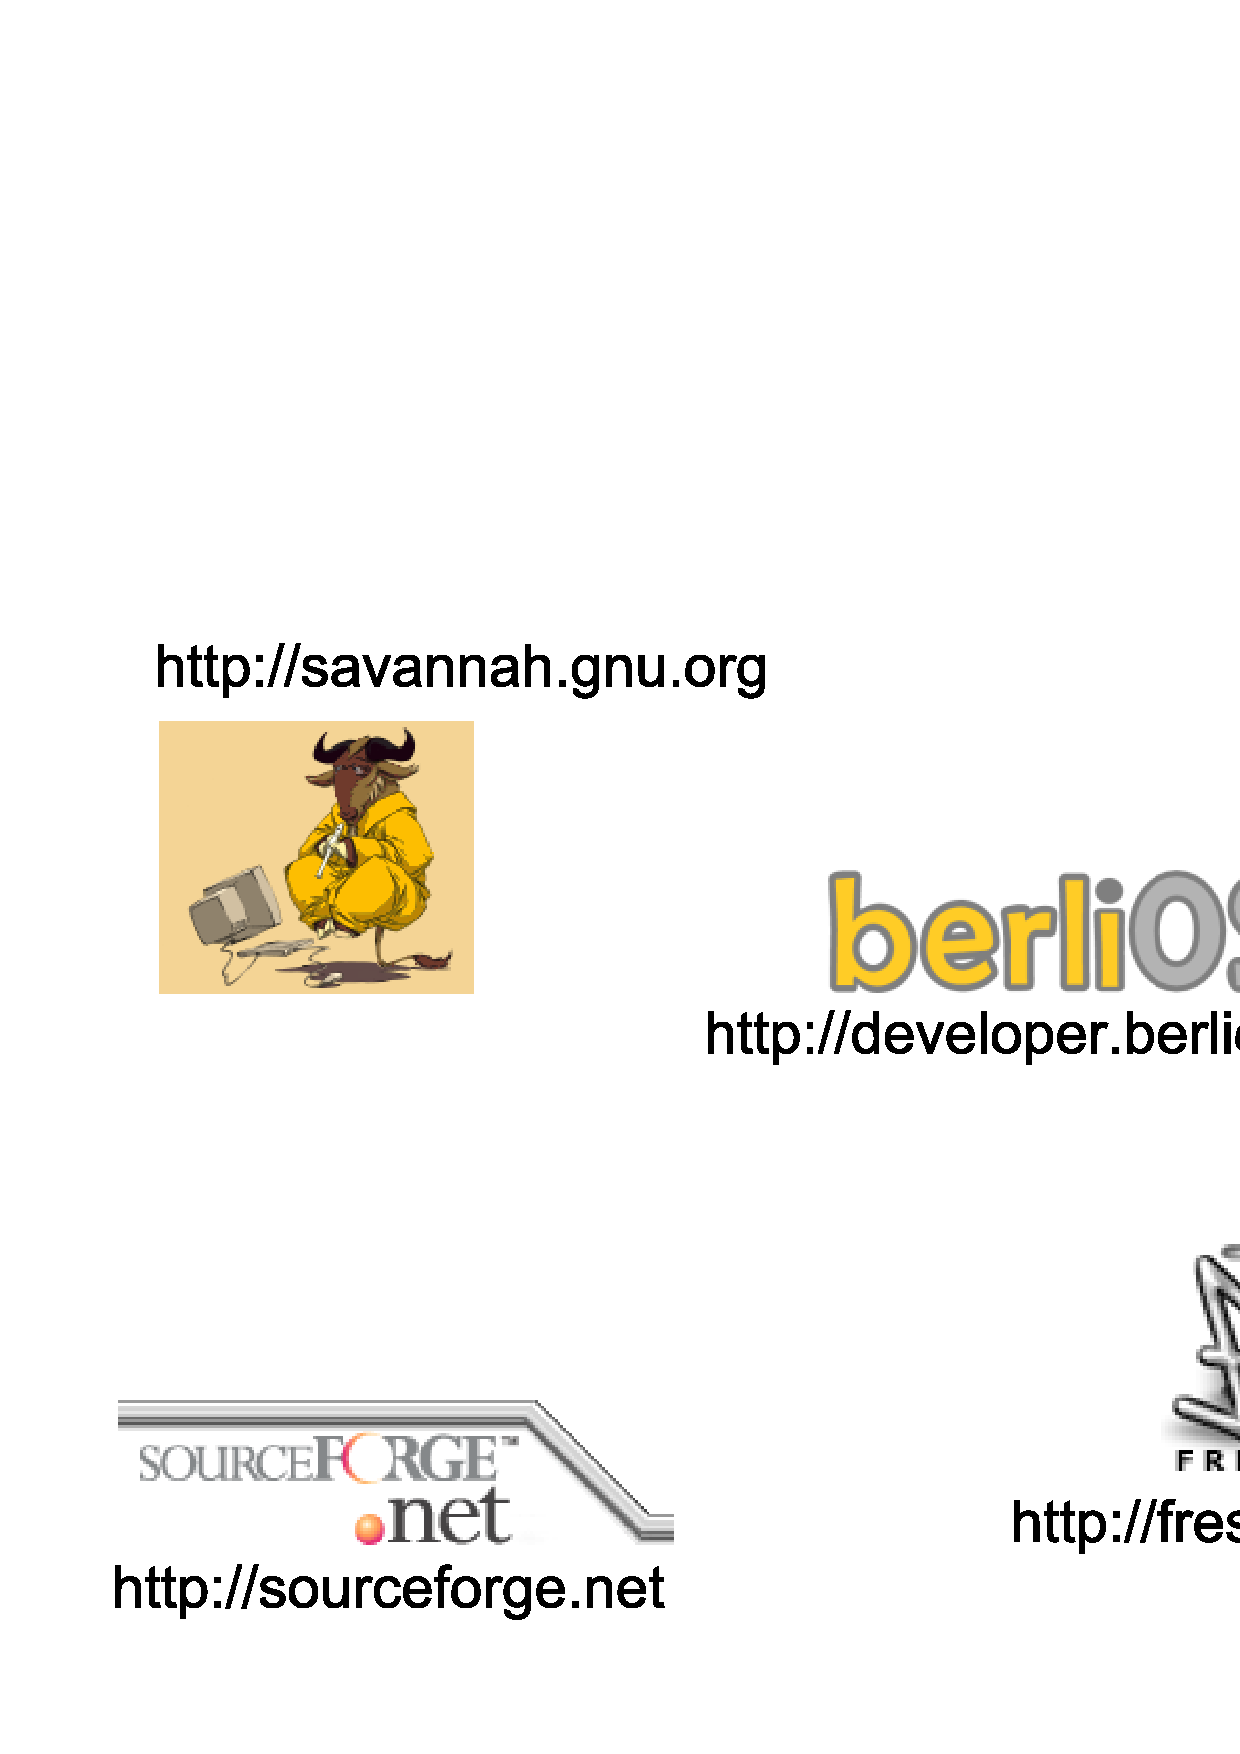
\includegraphics[scale=0.3,angle=-90]{graphic/portals.pdf}
        \caption{FLOSS Development Portals}
        \label{portals_figure}
    \end{center}
\end{figure}

As \emph{BerliOS} states in its slogan, it is the aim of development portals of
that kind to \textit{foster open source development}. In \emph{Savannah's}
words, they are \textit{central points for the development, distribution and
maintenance of FLOSS}. Although very often supported by well-known sponsors,
most portals are and want to stay independent. Using them, OSS projects and their
developers are offered several free services (figure \ref{services_figure}).
Since not all of these are always useful, projects can configure their portal
sites as needed.

\begin{figure}[ht]
    \begin{center}
        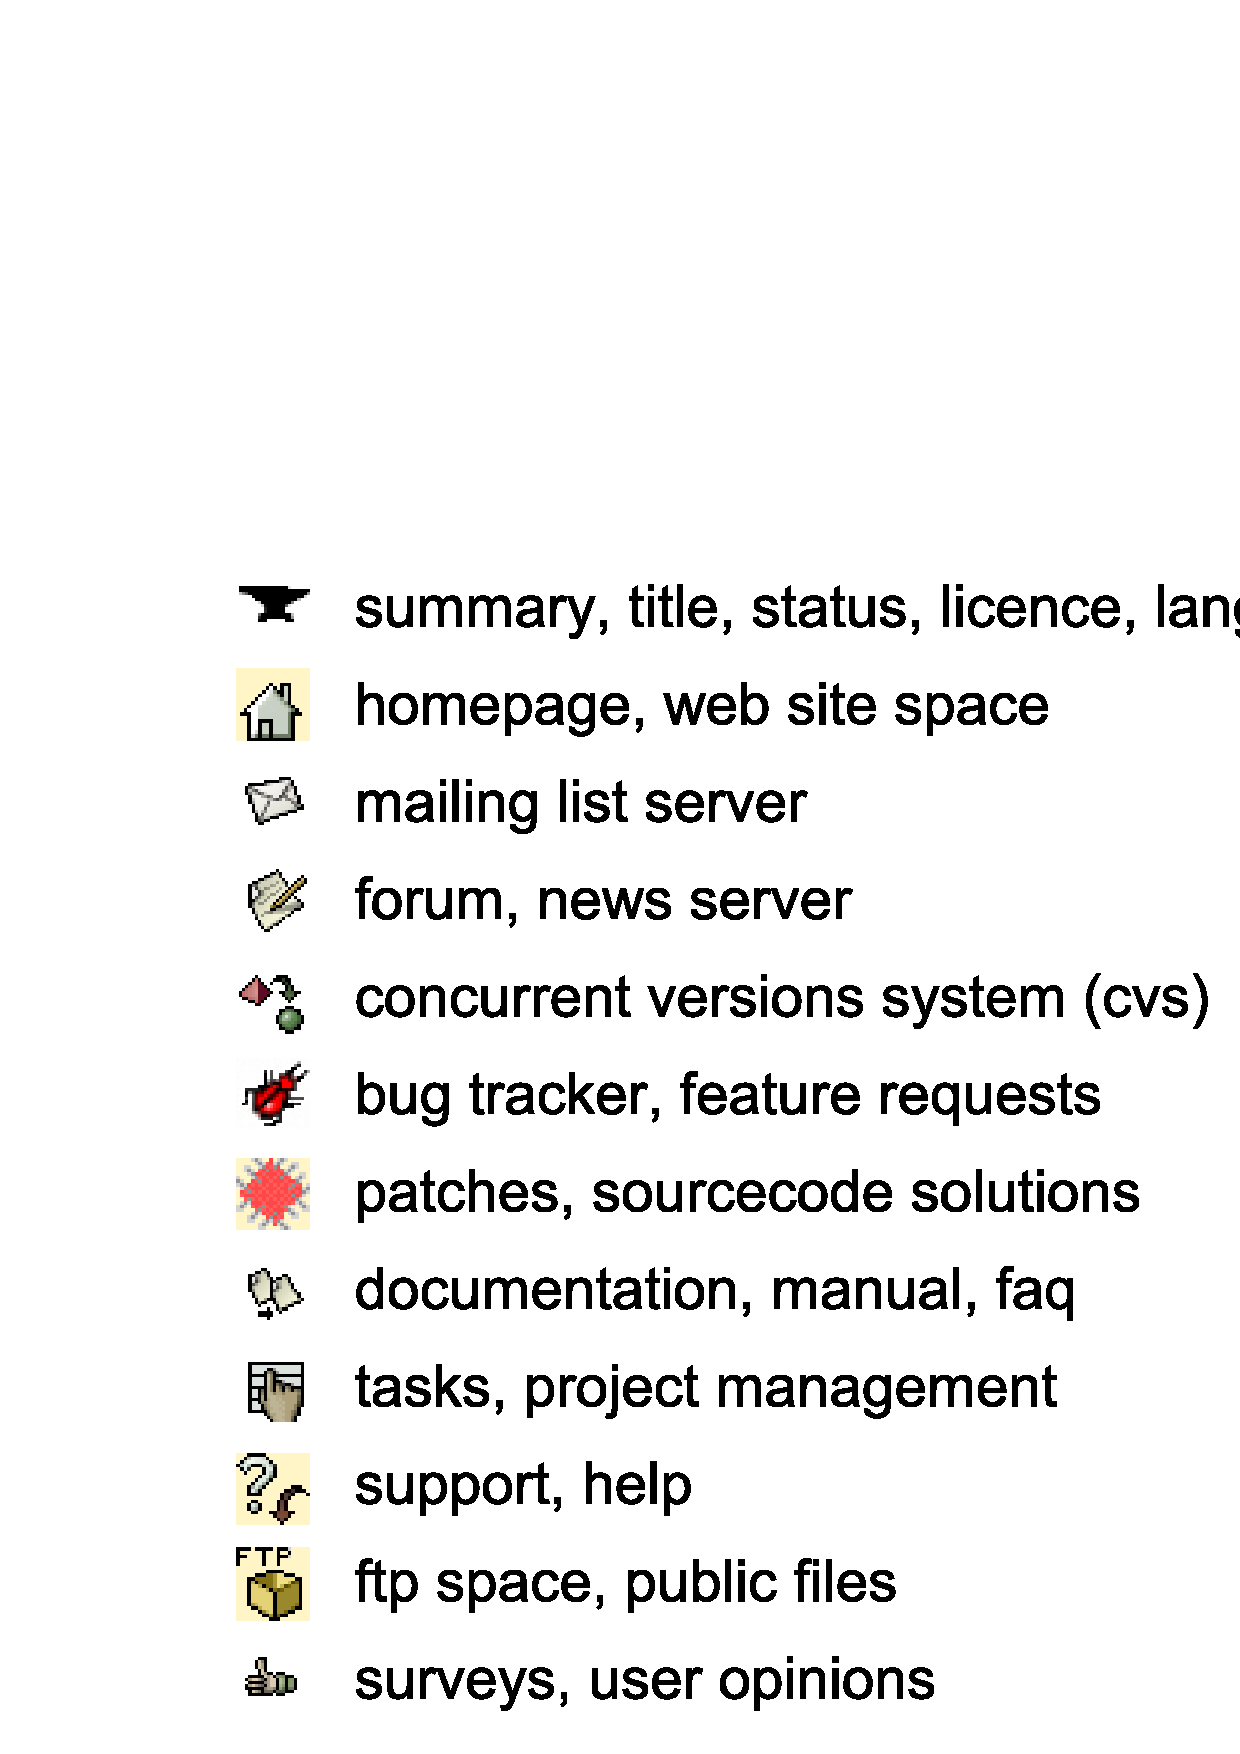
\includegraphics[scale=0.3,angle=-90]{graphic/services.pdf}
        \caption{Portal Services}
        \label{services_figure}
    \end{center}
\end{figure}

\emph{Res Medicinae} was one of the first OSS projects registered at
Sourceforge (number 4237 of now more than 100,000). CYBOP (CYBOL, CYBOI) is
hosted at BerliOS.
